% Diagram metode SSR-RCUS (Li dkk., AAAI 2026), gaya sama dengan arsitektur_medium.tex.
% Kompilasi (dari folder ini): pdflatex ssr_rcus.tex && pdftoppm -png -r 300 -singlefile ssr_rcus.pdf ssr_rcus
\documentclass[border=6pt]{standalone}
\usepackage{amssymb}
\usepackage{mathptmx}
\usepackage{tikz}
\usetikzlibrary{arrows.meta, shadows, calc, positioning}

\definecolor{ink}{HTML}{3A3936}
\definecolor{muted}{HTML}{8A8984}
\definecolor{dataF}{HTML}{F0EFEC}
\definecolor{modelE}{HTML}{2A78D6}\definecolor{modelF}{HTML}{DCE9F9}
\definecolor{augE}{HTML}{EB6834}\definecolor{augF}{HTML}{FDE3D6}
\definecolor{opE}{HTML}{6250D6}\definecolor{opF}{HTML}{EBE9FB}
\definecolor{lossE}{HTML}{1BAF7A}\definecolor{lossF}{HTML}{D9F3E9}

\tikzset{
  every node/.style={font=\small, text=ink, align=center},
  base/.style={rectangle, rounded corners=3pt, minimum height=12mm, inner sep=3pt, line width=0.8pt},
  data/.style={base, fill=dataF, draw=muted, text width=22mm},
  model/.style={base, fill=modelF, draw=modelE, text width=22mm},
  aug/.style={base, fill=augF, draw=augE, line width=1.2pt, text width=31mm},
  outp/.style={base, fill=opF, draw=opE, text width=27mm},
  loss/.style={base, fill=lossF, draw=lossE, text width=31mm},
  plain/.style={base, fill=dataF, draw=muted, text width=31mm},
  tensor/.style={rectangle, fill=white, draw=modelE, line width=0.8pt, minimum width=6mm, minimum height=8.5mm,
                 double copy shadow={shadow xshift=1.6pt, shadow yshift=1.6pt, draw=modelE, fill=white}},
  flow/.style={-{Stealth[length=2.3mm]}, line width=0.8pt, draw=ink, rounded corners=4pt},
  note/.style={font=\footnotesize\itshape, text=muted},
}

\newcommand{\sub}{\footnotesize\color{muted}}
\begin{document}
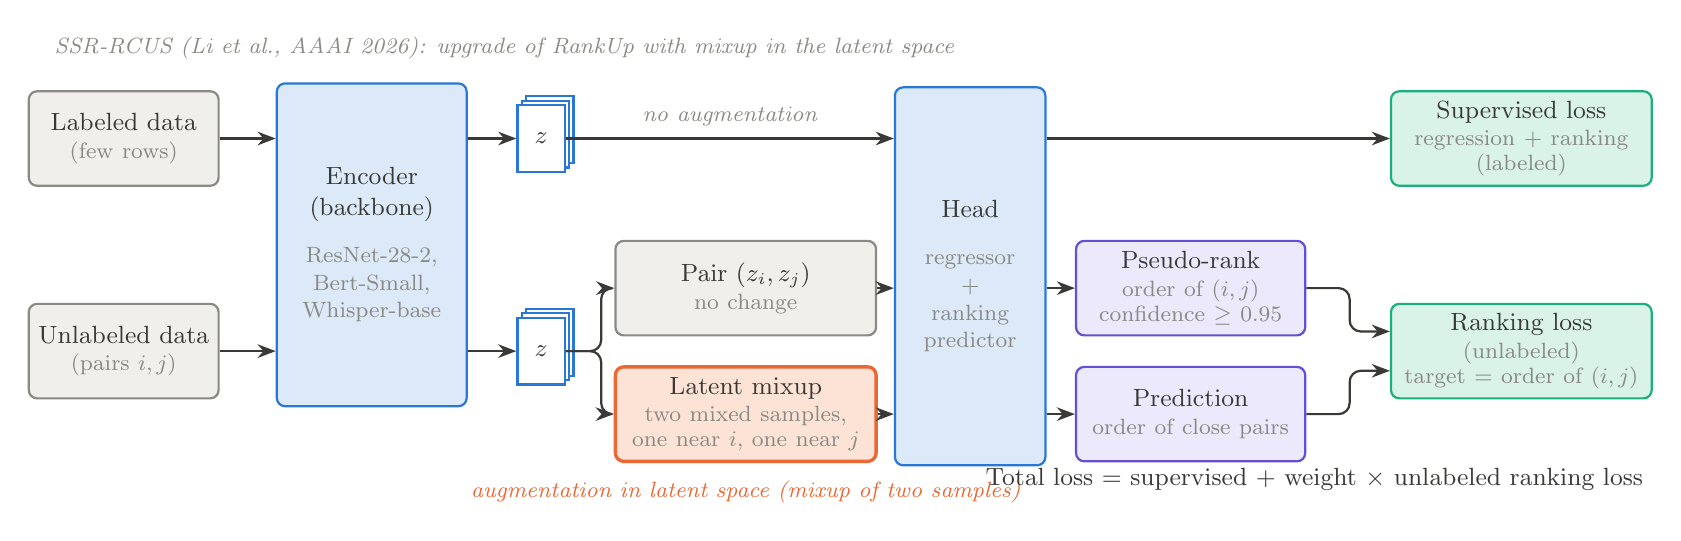
\begin{tikzpicture}
\def\yL{0} \def\yU{-2.7} \def\yW{-1.9} \def\yS{-3.5}

\node[note, anchor=west] at (-1.0,1.15) {SSR-RCUS (Li et al., AAAI 2026): upgrade of RankUp with mixup in the latent space};

\node[data] (xl) at (0,\yL) {Labeled data\\[-1pt]{\sub (few rows)}};
\node[data] (xu) at (0,\yU) {Unlabeled data\\[-1pt]{\sub (pairs $i,j$)}};

\node[model, minimum height=41mm] (enc) at (3.15,-1.35)
  {Encoder\\(backbone)\\[6pt]{\sub ResNet-28-2,}\\[-1pt]{\sub Bert-Small,}\\[-1pt]{\sub Whisper-base}};
\node[tensor] (hl) at (5.3,\yL) {$z$};
\node[tensor] (hu) at (5.3,\yU) {$z$};

\node[plain] (aw) at (7.9,\yW) {Pair $(z_i, z_j)$\\[-1pt]{\sub no change}};
\node[aug] (as) at (7.9,\yS) {Latent mixup\\[-1pt]{\sub two mixed samples,}\\[-2pt]{\sub one near $i$, one near $j$}};

\node[model, text width=17mm, minimum height=48mm] (head) at (10.75,-1.75)
  {Head\\[6pt]{\sub regressor}\\[-1pt]{\sub +}\\[-1pt]{\sub ranking}\\[-1pt]{\sub predictor}};

\node[outp] (pl) at (13.55,\yW) {Pseudo-rank\\[-1pt]{\sub order of $(i,j)$}\\[-2pt]{\sub confidence $\ge 0.95$}};
\node[outp] (pr) at (13.55,\yS) {Prediction\\[-1pt]{\sub order of close pairs}};
\node[loss] (lc) at (17.75,\yU) {Ranking loss\\[-1pt]{\sub (unlabeled)}\\[-2pt]{\sub target = order of $(i,j)$}};
\node[loss] (ls) at (17.75,\yL) {Supervised loss\\[-1pt]{\sub regression + ranking}\\[-2pt]{\sub (labeled)}};

\draw[flow] (xl) -- (xl -| enc.west);
\draw[flow] (xu) -- (xu -| enc.west);
\draw[flow] (enc.east |- hl) -- (hl);
\draw[flow] (enc.east |- hu) -- (hu);
\draw[flow] (hl) -- node[note, above=1pt] {no augmentation} (hl -| head.west);
\draw[flow] (hu.east) -- ++(0.45,0) |- (aw.west);
\draw[flow] (hu.east) -- ++(0.45,0) |- (as.west);
\draw[flow] (aw) -- (aw -| head.west);
\draw[flow] (as) -- (as -| head.west);
\draw[flow] (head.east |- ls) -- (ls);
\draw[flow] (head.east |- pl) -- (pl);
\draw[flow] (head.east |- pr) -- (pr);
\draw[flow] (pl.east) -- ++(0.55,0) |- ([yshift=2.5mm]lc.west);
\draw[flow] (pr.east) -- ++(0.55,0) |- ([yshift=-2.5mm]lc.west);

\node[font=\footnotesize\itshape, text=augE, below=3pt] at (as.south) {augmentation in latent space (mixup of two samples)};
\node[anchor=north east] at ($(lc.south east)+(0,-0.75)$)
  {Total loss $=$ supervised $+$ weight $\times$ unlabeled ranking loss};
\end{tikzpicture}
\end{document}
